\begin{figure*}[ht]
\subfigure[]{
 \resizebox{0.4\textwidth}{!}{
\scalebox{.4}{
\schemestart
0 \arrow(0--$y_{s0}$){<=>[$\mathrm{k_{on}}$][$\mathrm{k_{off}}$]}[,,,red] $y_{s0}$
\arrow{<=>[$u^S$][$d^S$]}[90,,,red] 
$x_{s0}$ \arrow($x_{s0}$--$x_{s1}$){->[$f$]}[,,,red]$x_{s1}$
\arrow(@$y_{s0}$--$y_{s1}$){<-[][$b$]}[,,,red] $y_{s1}$ \arrow{<=>[$u^S$][$d^S$]}[90,,,red]
\arrow(@$y_{s1}$--$y_{s2}$){<-[][$b$]}[,,,red] $y_{s2}$
\arrow{<=>[$u^S$][$d^S$]}[90,,,red] 
\arrow(@$x_{s1}$--$x_{s2}$){->[$f$]}[,,,red] $x_{s2}$
\schemestop}
}} 
\subfigure[]{
\resizebox{0.4\textwidth}{!}{
% This file was created by matlab2tikz.
%
%The latest updates can be retrieved from
%  http://www.mathworks.com/matlabcentral/fileexchange/22022-matlab2tikz-matlab2tikz
%where you can also make suggestions and rate matlab2tikz.
%
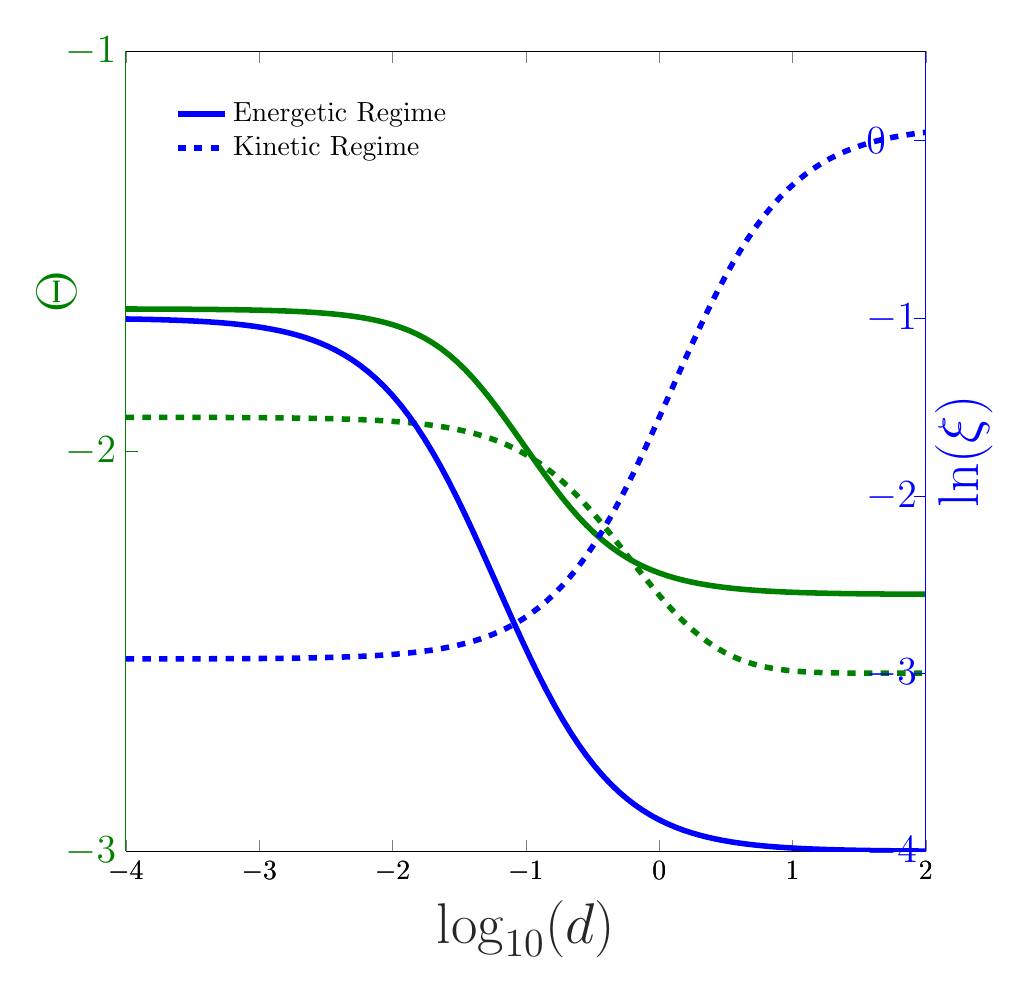
\begin{tikzpicture}


\begin{axis}[%
width=4in,
height=4in,
at={(0in,0in)},
scale only axis,
xmin=-4,
xmax=2,
xlabel style={font=\huge\color{white!15!black}},
xlabel={$\log_{10}(d)$},
separate axis lines,
axis y line*=left,
every outer y axis line/.append style={black!50!green},
every y tick label/.append style={font=\Large\color{black!50!green}},
every y tick/.append style={black!50!green},
ymin=-3,
ymax=-1,
ytick={-3, -2, -1},
ylabel style={font=\huge\color{black!50!green}, at={(axis description cs:-0.05,0.7)}},
ylabel={$\Theta$},
axis background/.style={fill=none},
yticklabel pos=right,
]

\addplot [color=black!50!green, line width=2.0pt]
  table[row sep=crcr]{%
-4	-1.64399326616915\\
-3.93939393939394	-1.64404192835098\\
-3.87878787878788	-1.64409793618038\\
-3.81818181818182	-1.64416240826328\\
-3.75757575757576	-1.6442366366041\\
-3.6969696969697	-1.64432211441953\\
-3.63636363636364	-1.64442056868828\\
-3.57575757575758	-1.64453399831721\\
-3.51515151515152	-1.64466471898601\\
-3.45454545454545	-1.64481541595269\\
-3.39393939393939	-1.64498920637236\\
-3.33333333333333	-1.64518971300906\\
-3.27272727272727	-1.64542115161907\\
-3.21212121212121	-1.64568843476475\\
-3.15151515151515	-1.64599729539496\\
-3.09090909090909	-1.64635443421425\\
-3.03030303030303	-1.64676769566845\\
-2.96969696969697	-1.64724627830413\\
-2.90909090909091	-1.64780098630998\\
-2.84848484848485	-1.64844453019668\\
-2.78787878787879	-1.64919188577388\\
-2.72727272727273	-1.65006072175416\\
-2.66666666666667	-1.65107190731864\\
-2.60606060606061	-1.65225011161501\\
-2.54545454545455	-1.6536245071292\\
-2.48484848484848	-1.65522958777301\\
-2.42424242424242	-1.65710610980957\\
-2.36363636363636	-1.65930215865735\\
-2.3030303030303	-1.66187433614615\\
-2.24242424242424	-1.66488904945341\\
-2.18181818181818	-1.66842386241833\\
-2.12121212121212	-1.67256883854191\\
-2.06060606060606	-1.67742775702973\\
-2	-1.68311901075324\\
-1.93939393939394	-1.68977588930481\\
-1.87878787878788	-1.69754580781161\\
-1.81818181818182	-1.70658787733804\\
-1.75757575757576	-1.71706807838909\\
-1.6969696969697	-1.72915130506177\\
-1.63636363636364	-1.74298985336353\\
-1.57575757575758	-1.75870867512171\\
-1.51515151515152	-1.77638889315987\\
-1.45454545454545	-1.79605234958365\\
-1.39393939393939	-1.8176506943523\\
-1.33333333333333	-1.84106203380798\\
-1.27272727272727	-1.86609623609104\\
-1.21212121212121	-1.8925072698768\\
-1.15151515151515	-1.92000875215079\\
-1.09090909090909	-1.94828843522621\\
-1.03030303030303	-1.97701897326746\\
-0.96969696969697	-2.00586505820671\\
-0.909090909090909	-2.0344893131226\\
-0.848484848484849	-2.06255991008871\\
-0.787878787878788	-2.08976156016614\\
-0.727272727272727	-2.11580923915707\\
-0.666666666666667	-2.14046212308555\\
-0.606060606060606	-2.1635346348534\\
-0.545454545454545	-2.18490230024756\\
-0.484848484848485	-2.20450164703108\\
-0.424242424242424	-2.22232486634054\\
-0.363636363636364	-2.23841087687506\\
-0.303030303030303	-2.25283467732429\\
-0.242424242424242	-2.26569661256779\\
-0.181818181818182	-2.27711267826629\\
-0.121212121212121	-2.2872064658982\\
-0.0606060606060606	-2.2961029304659\\
0	-2.30392388545994\\
0.0606060606060605	-2.31078498148072\\
0.121212121212121	-2.31679387197855\\
0.181818181818182	-2.32204927589366\\
0.242424242424242	-2.32664068379999\\
0.303030303030303	-2.33064850205503\\
0.363636363636363	-2.33414447707813\\
0.424242424242424	-2.33719228365249\\
0.484848484848484	-2.33984819512561\\
0.545454545454546	-2.34216177962075\\
0.606060606060606	-2.34417658584804\\
0.666666666666667	-2.34593079609861\\
0.727272727272728	-2.34745783377239\\
0.787878787878788	-2.34878691941395\\
0.848484848484849	-2.34994357358098\\
0.909090909090909	-2.35095006761689\\
0.96969696969697	-2.35182582503789\\
1.03030303030303	-2.35258777713554\\
1.09090909090909	-2.35325067679274\\
1.15151515151515	-2.35382737459139\\
1.21212121212121	-2.35432906117542\\
1.27272727272727	-2.35476547960479\\
1.33333333333333	-2.35514511114961\\
1.39393939393939	-2.35547533766224\\
1.45454545454545	-2.35576258335295\\
1.51515151515152	-2.35601243849333\\
1.57575757575758	-2.35622976728937\\
1.63636363636364	-2.35641880190706\\
1.6969696969697	-2.35658322439742\\
1.75757575757576	-2.35672623805702\\
1.81818181818182	-2.35685062957085\\
1.87878787878788	-2.35695882311754\\
1.93939393939394	-2.35705292746852\\
2	-2.35713477698292\\
};

\addplot [color=black!50!green, dashed, line width=2.0pt]
  table[row sep=crcr]{%
-4	-1.91481446824113\\
-3.93939393939394	-1.9148298348327\\
-3.87878787878788	-1.91484750214673\\
-3.81818181818182	-1.91486781456116\\
-3.75757575757576	-1.9148911679718\\
-3.6969696969697	-1.91491801748972\\
-3.63636363636364	-1.91494888628565\\
-3.57575757575758	-1.91498437575135\\
-3.51515151515152	-1.91502517717279\\
-3.45454545454545	-1.9150720851381\\
-3.39393939393939	-1.91512601293614\\
-3.33333333333333	-1.915188010238\\
-3.27272727272727	-1.91525928339577\\
-3.21212121212121	-1.91534121874103\\
-3.15151515151515	-1.91543540931892\\
-3.09090909090909	-1.91554368555538\\
-3.03030303030303	-1.91566815042374\\
-2.96969696969697	-1.91581121975437\\
-2.90909090909091	-1.91597566841799\\
-2.84848484848485	-1.91616468320962\\
-2.78787878787879	-1.91638192336725\\
-2.72727272727273	-1.91663158977664\\
-2.66666666666667	-1.91691850404158\\
-2.60606060606061	-1.91724819873643\\
-2.54545454545455	-1.91762702030312\\
-2.48484848484848	-1.91806224620511\\
-2.42424242424242	-1.9185622181021\\
-2.36363636363636	-1.91913649295328\\
-2.3030303030303	-1.91979601408463\\
-2.24242424242424	-1.92055330435133\\
-2.18181818181818	-1.92142268356949\\
-2.12121212121212	-1.92242051235236\\
-2.06060606060606	-1.9235654643254\\
-2	-1.92487882835762\\
-1.93939393939394	-1.92638484185953\\
-1.87878787878788	-1.92811105526463\\
-1.81818181818182	-1.93008872640228\\
-1.75757575757576	-1.93235324141957\\
-1.6969696969697	-1.93494455600534\\
-1.63636363636364	-1.93790764664566\\
-1.57575757575758	-1.94129295617461\\
-1.51515151515152	-1.94515681060063\\
-1.45454545454545	-1.94956177467814\\
-1.39393939393939	-1.95457690155718\\
-1.33333333333333	-1.96027781678382\\
-1.27272727272727	-1.96674655890967\\
-1.21212121212121	-1.97407107849447\\
-1.15151515151515	-1.98234427578118\\
-1.09090909090909	-1.99166243770874\\
-1.03030303030303	-2.00212292231591\\
-0.96969696969697	-2.01382094097902\\
-0.909090909090909	-2.02684531758016\\
-0.848484848484849	-2.0412731725577\\
-0.787878787878788	-2.0571636029392\\
-0.727272727272727	-2.07455061550642\\
-0.666666666666667	-2.09343581287762\\
-0.606060606060606	-2.1137815982259\\
-0.545454545454545	-2.13550588368954\\
-0.484848484848485	-2.15847935675654\\
-0.424242424242424	-2.18252616925136\\
-0.363636363636364	-2.20742841036492\\
-0.303030303030303	-2.2329339806899\\
-0.242424242424242	-2.25876673347223\\
-0.181818181818182	-2.28463732632825\\
-0.121212121212121	-2.31025338587006\\
-0.0606060606060606	-2.3353283002312\\
0	-2.35958884925627\\
0.0606060606060605	-2.38278243596321\\
0.121212121212121	-2.40468456319652\\
0.181818181818182	-2.4251065017565\\
0.242424242424242	-2.44390228323638\\
0.303030303030303	-2.46097373689577\\
0.363636363636363	-2.47627250982277\\
0.424242424242424	-2.48979869935911\\
0.484848484848484	-2.50159647984848\\
0.545454545454546	-2.51174756838448\\
0.606060606060606	-2.5203634512702\\
0.666666666666667	-2.52757712965795\\
0.727272727272728	-2.53353494628937\\
0.787878787878788	-2.53838893437811\\
0.848484848484849	-2.54229006820927\\
0.909090909090909	-2.54538272584727\\
0.96969696969697	-2.54780055756955\\
1.03030303030303	-2.54966380027753\\
1.09090909090909	-2.55107792783941\\
1.15151515151515	-2.55213341662683\\
1.21212121212121	-2.55290635063319\\
1.27272727272727	-2.5534595874259\\
1.33333333333333	-2.55384423921235\\
1.39393939393939	-2.55410127462338\\
1.45454545454545	-2.55426310194179\\
1.51515151515152	-2.55435504423941\\
1.57575757575758	-2.55439665689\\
1.63636363636364	-2.5544028672841\\
1.6969696969697	-2.554384936331\\
1.75757575757576	-2.55435125337981\\
1.81818181818182	-2.55430798254559\\
1.87878787878788	-2.55425958087953\\
1.93939393939394	-2.55420920879764\\
2	-2.55415905172779\\
};

\end{axis}

\begin{axis}[%
width=4in,
height=4in,
at={(0in,0in)},
scale only axis,
xmin=-4,
xmax=2,
xlabel style={font=\huge\color{white!15!black}},
%xlabel={$\log(d)$},
separate axis lines,
axis y line*=right,
every outer y axis line/.append style={blue},
every y tick label/.append style={font=\Large\color{blue}},
every y tick/.append style={blue},
ymin=-4,
ymax=0.5,
ytick={-4, -3, -2, -1, 0},
ylabel style={font=\huge\color{blue}},
ylabel={$\ln(\xi)$},
y tick label style={xshift={-2.5em},anchor=west},
axis background/.style={fill=none},
yticklabel pos=right,
legend style={at={(0.05,0.85)}, anchor=south west, legend cell align=left, align=left, fill=none, draw=none}
]
\addplot [color=blue, line width=2.0pt]
  table[row sep=crcr]{%
-4	-1.00514528094671\\
-3.93939393939394	-1.00591417966106\\
-3.87878787878788	-1.00679769874349\\
-3.81818181818182	-1.00781283426098\\
-3.75757575757576	-1.00897907348236\\
-3.6969696969697	-1.01031875073412\\
-3.63636363636364	-1.01185745110524\\
-3.57575757575758	-1.01362446746407\\
-3.51515151515152	-1.01565331654621\\
-3.45454545454545	-1.01798232005898\\
-3.39393939393939	-1.02065525676499\\
-3.33333333333333	-1.0237220912662\\
-3.27272727272727	-1.02723978462868\\
-3.21212121212121	-1.03127319090066\\
-3.15151515151515	-1.03589604184445\\
-3.09090909090909	-1.04119201958538\\
-3.03030303030303	-1.04725591313774\\
-2.96969696969697	-1.05419484957228\\
-2.90909090909091	-1.06212958358863\\
-2.84848484848485	-1.07119582004068\\
-2.78787878787879	-1.08154553210583\\
-2.72727272727273	-1.09334822287825\\
-2.66666666666667	-1.10679205985796\\
-2.60606060606061	-1.12208478993182\\
-2.54545454545455	-1.13945431712213\\
-2.48484848484848	-1.15914879722334\\
-2.42424242424242	-1.18143607377528\\
-2.36363636363636	-1.20660225092131\\
-2.3030303030303	-1.23494917412145\\
-2.24242424242424	-1.26679057444976\\
-2.18181818181818	-1.30244663289609\\
-2.12121212121212	-1.34223674568556\\
-2.06060606060606	-1.38647032888462\\
-2	-1.43543559883289\\
-1.93939393939394	-1.48938641030531\\
-1.87878787878788	-1.54852742808911\\
-1.81818181818182	-1.61299814355508\\
-1.75757575757576	-1.68285650931167\\
-1.6969696969697	-1.75806322401915\\
-1.63636363636364	-1.83846791692171\\
-1.57575757575758	-1.9237986117283\\
-1.51515151515152	-2.01365584664532\\
-1.45454545454545	-2.10751265658967\\
-1.39393939393939	-2.20472127100837\\
-1.33333333333333	-2.30452686214559\\
-1.27272727272727	-2.4060880428896\\
-1.21212121212121	-2.50850313827492\\
-1.15151515151515	-2.61084063524474\\
-1.09090909090909	-2.71217174610758\\
-1.03030303030303	-2.81160277769924\\
-0.96969696969697	-2.90830502080043\\
-0.909090909090909	-3.00154015910906\\
-0.848484848484849	-3.09067969712817\\
-0.787878787878788	-3.17521754181492\\
-0.727272727272727	-3.25477554766662\\
-0.666666666666667	-3.32910245591022\\
-0.606060606060606	-3.39806715201836\\
-0.545454545454545	-3.46164748844058\\
-0.484848484848485	-3.51991606070038\\
-0.424242424242424	-3.57302430296156\\
-0.363636363636364	-3.62118612131327\\
-0.303030303030303	-3.66466205561363\\
-0.242424242424242	-3.70374469886533\\
-0.181818181818182	-3.73874584424297\\
-0.121212121212121	-3.76998560008697\\
-0.0606060606060606	-3.79778352731955\\
0	-3.82245171631547\\
0.0606060606060605	-3.84428962941829\\
0.121212121212121	-3.86358048405467\\
0.181818181818182	-3.88058893117624\\
0.242424242424242	-3.89555978658208\\
0.303030303030303	-3.90871758951584\\
0.363636363636363	-3.92026678876241\\
0.424242424242424	-3.93039238562434\\
0.484848484848484	-3.93926089283758\\
0.545454545454546	-3.9470214959465\\
0.606060606060606	-3.95380732814733\\
0.666666666666667	-3.959736792711\\
0.727272727272728	-3.96491488266595\\
0.787878787878788	-3.96943446101102\\
0.848484848484849	-3.973377483421\\
0.909090909090909	-3.97681613357599\\
0.96969696969697	-3.97981389066919\\
1.03030303030303	-3.98242651060806\\
1.09090909090909	-3.9847028629193\\
1.15151515151515	-3.98668577994793\\
1.21212121212121	-3.98841269880268\\
1.27272727272727	-3.98991648551135\\
1.33333333333333	-3.99122571565551\\
1.39393939393939	-3.99236533651757\\
1.45454545454545	-3.99335723249601\\
1.51515151515152	-3.99422049656245\\
1.57575757575758	-3.99497302431736\\
1.63636363636364	-3.99562730771617\\
1.6969696969697	-3.99619844791424\\
1.75757575757576	-3.99668129038028\\
1.81818181818182	-3.99712192780194\\
1.87878787878788	-3.99748647550716\\
1.93939393939394	-3.99786080870592\\
2	-3.99808968513925\\
};
\addlegendentry{Energetic Regime}

\addplot [color=blue, dashed, line width=2.0pt]
  table[row sep=crcr]{%
-4	-2.91733526286331\\
-3.93939393939394	-2.91729665488815\\
-3.87878787878788	-2.9172523331581\\
-3.81818181818182	-2.91720127268045\\
-3.75757575757576	-2.91714268818111\\
-3.6969696969697	-2.9170752463596\\
-3.63636363636364	-2.91699769207382\\
-3.57575757575758	-2.91690860022524\\
-3.51515151515152	-2.91680611008076\\
-3.45454545454545	-2.9166882797432\\
-3.39393939393939	-2.91655286015101\\
-3.33333333333333	-2.91639716700639\\
-3.27272727272727	-2.9162182235781\\
-3.21212121212121	-2.91601240550786\\
-3.15151515151515	-2.91577587944173\\
-3.09090909090909	-2.91550394190394\\
-3.03030303030303	-2.91519134182915\\
-2.96969696969697	-2.91483206628571\\
-2.90909090909091	-2.91441904590452\\
-2.84848484848485	-2.91394435382346\\
-2.78787878787879	-2.91339880870926\\
-2.72727272727273	-2.91277178955527\\
-2.66666666666667	-2.91205120524763\\
-2.60606060606061	-2.9112232006956\\
-2.54545454545455	-2.91027178413835\\
-2.48484848484848	-2.90917870141141\\
-2.42424242424242	-2.90792299308768\\
-2.36363636363636	-2.90648064348341\\
-2.3030303030303	-2.90482416309134\\
-2.24242424242424	-2.90292205389708\\
-2.18181818181818	-2.90073833735418\\
-2.12121212121212	-2.8982317585911\\
-2.06060606060606	-2.89535555974875\\
-2	-2.89205598242962\\
-1.93939393939394	-2.88827202718007\\
-1.87878787878788	-2.88393422752991\\
-1.81818181818182	-2.87896370481408\\
-1.75757575757576	-2.87327099099649\\
-1.6969696969697	-2.86675483431648\\
-1.63636363636364	-2.85930108985984\\
-1.57575757575758	-2.85078116591016\\
-1.51515151515152	-2.84105079330144\\
-1.45454545454545	-2.82994894009253\\
-1.39393939393939	-2.81729614981449\\
-1.33333333333333	-2.80289394873099\\
-1.27272727272727	-2.78652393901491\\
-1.21212121212121	-2.76794736456465\\
-1.15151515151515	-2.74690544553906\\
-1.09090909090909	-2.72312038052378\\
-1.03030303030303	-2.69629725719873\\
-0.96969696969697	-2.66612738985531\\
-0.909090909090909	-2.63229274569193\\
-0.848484848484849	-2.59447256036931\\
-0.787878787878788	-2.55235151278722\\
-0.727272727272727	-2.50562991252936\\
-0.666666666666667	-2.45403615697698\\
-0.606060606060606	-2.39734065674789\\
-0.545454545454545	-2.33537144498335\\
-0.484848484848485	-2.26803045132387\\
-0.424242424242424	-2.1953097212927\\
-0.363636363636364	-2.11730621909417\\
-0.303030303030303	-2.03423405260551\\
-0.242424242424242	-1.94643279032296\\
-0.181818181818182	-1.85437025025582\\
-0.121212121212121	-1.75863908276304\\
-0.0606060606060606	-1.65994626600367\\
0	-1.5590957150624\\
0.0606060606060605	-1.45696453421263\\
0.121212121212121	-1.35447427042031\\
0.181818181818182	-1.25255908536176\\
0.242424242424242	-1.15213298185254\\
0.303030303030303	-1.05405849188407\\
0.363636363636363	-0.959118954912089\\
0.424242424242424	-0.867996147764197\\
0.484848484848484	-0.781254438812565\\
0.545454545454546	-0.699331977944571\\
0.606060606060606	-0.622538760488771\\
0.666666666666667	-0.551060854058421\\
0.727272727272728	-0.484969675914825\\
0.787878787878788	-0.424234967497944\\
0.848484848484849	-0.368740076698282\\
0.909090909090909	-0.318298248440627\\
0.96969696969697	-0.27266881545735\\
1.03030303030303	-0.231572440573928\\
1.09090909090909	-0.194704819396904\\
1.15151515151515	-0.161748501216313\\
1.21212121212121	-0.132382693033455\\
1.27272727272727	-0.106291071286463\\
1.33333333333333	-0.0831677381019672\\
1.39393939393939	-0.062721527787329\\
1.45454545454545	-0.0446789024768589\\
1.51515151515152	-0.0287856831583516\\
1.57575757575758	-0.0148078508395435\\
1.63636363636364	-0.00253163043221874\\
1.6969696969697	0.00823695821086093\\
1.75757575757576	0.0176729273441505\\
1.81818181818182	0.0259334005293425\\
1.87878787878788	0.0331588443184213\\
1.93939393939394	0.0394743756237139\\
2	0.0449910875055136\\
};
\addlegendentry{Kinetic Regime}
\end{axis}

\end{tikzpicture}%
}} 
\subfigure[]{
 \resizebox{0.4\textwidth}{!}{
% This file was created by matlab2tikz.
%
%The latest updates can be retrieved from
%  http://www.mathworks.com/matlabcentral/fileexchange/22022-matlab2tikz-matlab2tikz
%where you can also make suggestions and rate matlab2tikz.
%
\definecolor{mycolor1}{rgb}{0.00000,0.000,0.000}%
%
\begin{tikzpicture}

\begin{axis}[%
width=4in,
height=4in,
at={(0in,0in)},
scale only axis,
xmin=-5,
xmax=5,
xtick={-4,-2,0,2,4},
xlabel style={font=\huge\color{white!15!black}},
xlabel={$\log_{10}(\omega_f)$},
separate axis lines,
axis y line*=left,
every outer y axis line/.append style={black!50!green},
every y tick label/.append style={font=\Large\color{black!50!green}},
every y tick/.append style={black!50!green},
ymin=-2.75,
ymax=-1.5,
ytick={-2.5, -2, -1.5},
ylabel style={font=\huge\color{black!50!green}, at={(axis description cs:-0.05,0.5)}},
ylabel={$\Theta$},
axis background/.style={fill=white},
yticklabel pos=right,
]
\addplot [color=black!50!green, line width=2.0pt, forget plot]
  table[row sep=crcr]{%
-5	-2.55980435421901\\
-4.79591836734694	-2.55980434186469\\
-4.59183673469388	-2.55980432209932\\
-4.38775510204082	-2.55980429047699\\
-4.18367346938776	-2.55980423988437\\
-3.97959183673469	-2.55980415893989\\
-3.77551020408163	-2.55980402943132\\
-3.57142857142857	-2.55980382221328\\
-3.36734693877551	-2.55980349063582\\
-3.16326530612245	-2.55980296001059\\
-2.95918367346939	-2.55980211070605\\
-2.75510204081633	-2.55980075096846\\
-2.55102040816327	-2.55979857309744\\
-2.3469387755102	-2.55979508245834\\
-2.14285714285714	-2.55978948167668\\
-1.93877551020408	-2.55978047965553\\
-1.73469387755102	-2.55976597146412\\
-1.53061224489796	-2.55974248912179\\
-1.3265306122449	-2.55970422882944\\
-1.12244897959184	-2.55964125714501\\
-0.918367346938776	-2.55953604663673\\
-0.714285714285714	-2.55935646634765\\
-0.510204081632653	-2.55904103103071\\
-0.306122448979592	-2.55846711374081\\
-0.102040816326531	-2.5573824631785\\
0.102040816326531	-2.55526283181266\\
0.306122448979592	-2.55104223244863\\
0.510204081632653	-2.54269657640861\\
0.714285714285714	-2.52686849980221\\
0.918367346938776	-2.49912348695541\\
1.12244897959184	-2.45540097667699\\
1.3265306122449	-2.39424027330782\\
1.53061224489796	-2.31872009496065\\
1.73469387755102	-2.23643351774748\\
1.93877551020408	-2.15689809777501\\
2.14285714285714	-2.08834622985733\\
2.3469387755102	-2.03500453117392\\
2.55102040816327	-1.99664670020636\\
2.75510204081633	-1.97050192502729\\
2.95918367346939	-1.95327271307917\\
3.16326530612245	-1.94215019118093\\
3.36734693877551	-1.93505897490393\\
3.57142857142857	-1.93057213060324\\
3.77551020408163	-1.92774632352692\\
3.97959183673469	-1.92597172389132\\
4.18367346938776	-1.92485925344566\\
4.38775510204082	-1.92416262937327\\
4.59183673469388	-1.92372670529494\\
4.79591836734694	-1.92345403508248\\
5	-1.92328352551524\\
};
\end{axis}

\begin{axis}[%
width=4in,
height=4in,
at={(0in,0in)},
scale only axis,
xmin=-5,
xmax=5,
xticklabels=\empty,
xlabel style={font=\huge\color{white!15!black}},
%xlabel={$\log(\omega_u)$},
separate axis lines,
axis y line*=right,
every outer y axis line/.append style={mycolor1},
every y tick label/.append style={font=\Large\color{mycolor1}},
every y tick/.append style={mycolor1},
ymin=-4,
ymax=-1,
ytick={-4, -3, -2, -1},
ylabel style={font=\huge\color{mycolor1}},
ylabel={$\log_{10}(\Delta S_i)$},
axis background/.style={fill=none},
yticklabel pos=right,
y tick label style={xshift={-3em},anchor=west},
legend style={at={(0.6,0.05)}, anchor=south west, legend cell align=left, align=left, fill=none, draw=none}
]

\addplot [color=blue, line width=2.0pt, forget plot]
  table[row sep=crcr]{%
-5	-1.00324296746153\\
-4.79591836734694	-1.00518467413702\\
-4.59183673469388	-1.00828549615505\\
-4.38775510204082	-1.01323202156867\\
-4.18367346938776	-1.02110924875673\\
-3.97959183673469	-1.03361913372891\\
-3.77551020408163	-1.05339987998379\\
-3.57142857142857	-1.08446353259473\\
-3.36734693877551	-1.13272573962688\\
-3.16326530612245	-1.20647977484271\\
-2.95918367346939	-1.31641151433184\\
-2.75510204081633	-1.47437574670688\\
-2.55102040816327	-1.68995928856333\\
-2.3469387755102	-1.96465461174935\\
-2.14285714285714	-2.28595937068162\\
-1.93877551020408	-2.62636142678962\\
-1.73469387755102	-2.95063990095384\\
-1.53061224489796	-3.22806606517476\\
-1.3265306122449	-3.44111528773649\\
-1.12244897959184	-3.58576962009024\\
-0.918367346938776	-3.66577229798171\\
-0.714285714285714	-3.68607304168395\\
-0.510204081632653	-3.64871549658509\\
-0.306122448979592	-3.55192606283928\\
-0.102040816326531	-3.39221649509467\\
0.102040816326531	-3.16896104158826\\
0.306122448979592	-2.88979991881088\\
0.510204081632653	-2.57367134356986\\
0.714285714285714	-2.24849026618408\\
0.918367346938776	-1.94372872033049\\
1.12244897959184	-1.68194322093462\\
1.3265306122449	-1.47391420758324\\
1.53061224489796	-1.31912683924617\\
1.73469387755102	-1.20982856438329\\
1.93877551020408	-1.13562465336114\\
2.14285714285714	-1.08663874885576\\
2.3469387755102	-1.05491500175665\\
2.55102040816327	-1.03463054724113\\
2.75510204081633	-1.02176752688542\\
2.95918367346939	-1.01365391259384\\
3.16326530612245	-1.00855333369983\\
3.36734693877551	-1.00535371204537\\
3.57142857142857	-1.00334927787622\\
3.77551020408163	-1.00209461395054\\
3.97959183673469	-1.00130969368936\\
4.18367346938776	-1.00081879269932\\
4.38775510204082	-1.00051189105748\\
4.59183673469388	-1.00031998008897\\
4.79591836734694	-1.00019988932097\\
5	-1.00012504294194\\
};

\addplot [color=mycolor1, line width=2.0pt]
  table[row sep=crcr]{%
-5	-10.4887860431965\\
-4.79591836734694	-10.018872539903\\
-4.59183673469388	-9.54896013053914\\
-4.38775510204082	-9.07904947305567\\
-4.18367346938776	-8.60914162277903\\
-3.97959183673469	-8.13923827509998\\
-3.77551020408163	-7.66934216049719\\
-3.57142857142857	-7.19945769439776\\
-3.36734693877551	-6.72959206421324\\
-3.16326530612245	-6.2597570963748\\
-2.95918367346939	-5.78997259808786\\
-2.75510204081633	-5.32027272040396\\
-2.55102040816327	-4.85071916882426\\
-2.3469387755102	-4.38143173349484\\
-2.14285714285714	-3.91266715686559\\
-1.93877551020408	-3.44504200926409\\
-1.73469387755102	-2.98018992353619\\
-1.53061224489796	-2.52264166503415\\
-1.3265306122449	-2.08444866987177\\
-1.12244897959184	-1.6925876678339\\
-0.918367346938776	-1.38830306242737\\
-0.714285714285714	-1.19858211900174\\
-0.510204081632653	-1.10535995600399\\
-0.306122448979592	-1.06547585927382\\
-0.102040816326531	-1.04581343344806\\
0.102040816326531	-1.02980553970525\\
0.306122448979592	-1.01005587372878\\
0.510204081632653	-0.983158591013787\\
0.714285714285714	-0.948488780440555\\
0.918367346938776	-0.908496812929897\\
1.12244897959184	-0.867974282063292\\
1.3265306122449	-0.831747825599495\\
1.53061224489796	-0.802623562292143\\
1.73469387755102	-0.781041528689259\\
1.93877551020408	-0.765953595199554\\
2.14285714285714	-0.755815899029205\\
2.3469387755102	-0.749180237964267\\
2.55102040816327	-0.744909709933227\\
2.75510204081633	-0.742190835610793\\
2.95918367346939	-0.740471635874598\\
3.16326530612245	-0.739389225872294\\
3.36734693877551	-0.738709582064917\\
3.57142857142857	-0.738283561967209\\
3.77551020408163	-0.738016799236848\\
3.97959183673469	-0.737849873722096\\
4.18367346938776	-0.737745461017099\\
4.38775510204082	-0.737680178531745\\
4.59183673469388	-0.737639353868555\\
4.79591836734694	-0.737613806101193\\
5	-0.737597883736549\\
};

\addplot [color=red, forget plot]
  table[row sep=crcr]{%
-0.714285714285714	-4\\
-0.714285714285714	-0.8\\
};

\addplot [color=red, forget plot, line width=2.5pt]
  table[row sep=crcr]{%
1.176	-3.9\\
1.176	-4.1\\
};
\end{axis}

\draw (6cm,0.1cm) node[above, text=blue, font=\fontsize{24}{24}\selectfont] 
      {$e^{-4\gamma}$};
      
      \draw (6.2cm,-0.6cm) node[above, text=red, font=\fontsize{18}{18}\selectfont] 
      {$d$};
      
\draw (9cm,9cm) node[above, text=blue, font=\fontsize{24}{24}\selectfont] 
      {$e^{-\gamma}$};

\end{tikzpicture}%
}} 
\subfigure[]{
\resizebox{0.4\textwidth}{!}{
% This file was created by matlab2tikz.
%
%The latest updates can be retrieved from
%  http://www.mathworks.com/matlabcentral/fileexchange/22022-matlab2tikz-matlab2tikz
%where you can also make suggestions and rate matlab2tikz.
%
\definecolor{mycolor1}{rgb}{0.00000,0.000,0.000}%
%
\begin{tikzpicture}

\begin{axis}[%
width=4in,
height=4in,
at={(0in,0in)},
scale only axis,
xmin=-5,
xmax=5.1,
xtick={-4,-2,0,2,4},
xlabel style={font=\huge\color{white!15!black}},
xlabel={$\log_{10}(\omega_d)$},
separate axis lines,
axis y line*=left,
every outer y axis line/.append style={black!50!green},
every y tick label/.append style={font=\Large\color{black!50!green}},
every y tick/.append style={black!50!green},
ymin=-2.75,
ymax=-1.5,
ytick={-2.5, -2, -1.5},
ylabel style={font=\huge\color{black!50!green}, at={(axis description cs:-0.05,0.5)}},
ylabel={$\Theta$},
axis background/.style={fill=white},
yticklabel pos=right,
]
\addplot [color=black!50!green, line width=2.0pt, forget plot]
  table[row sep=crcr]{%
-5	-2.06136739360636\\
-4.79591836734694	-2.06133098452498\\
-4.59183673469388	-2.06127281336862\\
-4.38775510204082	-2.06117994791906\\
-4.18367346938776	-2.06103188848541\\
-3.97959183673469	-2.06079632435536\\
-3.77551020408163	-2.06042280457035\\
-3.57142857142857	-2.05983378410276\\
-3.36734693877551	-2.05891327778527\\
-3.16326530612245	-2.05749624127166\\
-2.95918367346939	-2.0553704595266\\
-2.75510204081633	-2.05232604819149\\
-2.55102040816327	-2.04834502215962\\
-2.3469387755102	-2.04414631258541\\
-2.14285714285714	-2.04248721942915\\
-1.93877551020408	-2.0505517410539\\
-1.73469387755102	-2.08204007444239\\
-1.53061224489796	-2.15270075389332\\
-1.3265306122449	-2.26350648164775\\
-1.12244897959184	-2.38755767995892\\
-0.918367346938776	-2.48649709085836\\
-0.714285714285714	-2.54210400718391\\
-0.510204081632653	-2.56359568992166\\
-0.306122448979592	-2.56824778174746\\
-0.102040816326531	-2.56717996847928\\
0.102040816326531	-2.56498835199238\\
0.306122448979592	-2.5630669190242\\
0.510204081632653	-2.56166750297347\\
0.714285714285714	-2.560720419841\\
0.918367346938776	-2.56010156880124\\
1.12244897959184	-2.55970461831667\\
1.3265306122449	-2.55945263505503\\
1.53061224489796	-2.55929364366581\\
1.73469387755102	-2.55919368962833\\
1.93877551020408	-2.55913098933714\\
2.14285714285714	-2.55909171121751\\
2.3469387755102	-2.5590671263276\\
2.55102040816327	-2.55905174619163\\
2.75510204081633	-2.55904212759671\\
2.95918367346939	-2.55903611342884\\
3.16326530612245	-2.55903235345497\\
3.36734693877551	-2.55903000295637\\
3.57142857142857	-2.55902853364493\\
3.77551020408163	-2.55902761519728\\
3.97959183673469	-2.55902704109847\\
4.18367346938776	-2.55902668224787\\
4.38775510204082	-2.55902645794365\\
4.59183673469388	-2.55902631774003\\
4.79591836734694	-2.55902623010461\\
5	-2.55902617532746\\
};

\end{axis}

\begin{axis}[%
width=4in,
height=4in,
at={(0in,0in)},
scale only axis,
xmin=-5,
xmax=5.1,
xticklabels=\empty,
xlabel style={font=\huge\color{white!15!black}},
%xlabel={$\log(\omega_f)$},
separate axis lines,
axis y line*=right,
every outer y axis line/.append style={mycolor1},
every y tick label/.append style={font=\Large\color{mycolor1}},
every y tick/.append style={mycolor1},
ymin=-4,
ymax=-1,
ytick={-4, -3, -2, -1},
ylabel style={font=\huge\color{mycolor1}},
ylabel={$\log_{10}(\Delta S_i)$},
y tick label style={xshift={-3em},anchor=west},
axis background/.style={fill=none},
yticklabel pos=right,
legend style={at={(0.3,0.02)}, anchor=south west, legend cell align=left, align=left, fill=none, draw=none}
]
\addplot [color=blue, line width=2.0pt, forget plot]
  table[row sep=crcr]{%
-5	-1.00058857136098\\
-4.79591836734694	-1.00094149861245\\
-4.59183673469388	-1.00150592598248\\
-4.38775510204082	-1.0024084022304\\
-4.18367346938776	-1.00385088750123\\
-3.97959183673469	-1.00615521369432\\
-3.77551020408163	-1.00983301708543\\
-3.57142857142857	-1.01569459238005\\
-3.36734693877551	-1.02501544324557\\
-3.16326530612245	-1.03978388590852\\
-2.95918367346939	-1.06305128387009\\
-2.75510204081633	-1.09938396775195\\
-2.55102040816327	-1.15534232149406\\
-2.3469387755102	-1.23974008720114\\
-2.14285714285714	-1.36313548629773\\
-1.93877551020408	-1.53569753701758\\
-1.73469387755102	-1.76278232981669\\
-1.53061224489796	-2.03906365953137\\
-1.3265306122449	-2.34480701310853\\
-1.12244897959184	-2.64908419776115\\
-0.918367346938776	-2.92063044897484\\
-0.714285714285714	-3.13962761491161\\
-0.510204081632653	-3.30198856745968\\
-0.306122448979592	-3.4150640269815\\
-0.102040816326531	-3.49056609768521\\
0.102040816326531	-3.53966500827255\\
0.306122448979592	-3.57108998361989\\
0.510204081632653	-3.59101421059962\\
0.714285714285714	-3.60357613270272\\
0.918367346938776	-3.61146970760537\\
1.12244897959184	-3.61641975062493\\
1.3265306122449	-3.61952005759121\\
1.53061224489796	-3.62146035429933\\
1.73469387755102	-3.62267409494032\\
1.93877551020408	-3.62343311967073\\
2.14285714285714	-3.62390769600107\\
2.3469387755102	-3.6242043889115\\
2.55102040816327	-3.62438986038549\\
2.75510204081633	-3.62450579890251\\
2.95918367346939	-3.62457826890849\\
3.16326530612245	-3.62462357126198\\
3.36734693877551	-3.62465188356096\\
3.57142857142857	-3.62466958571435\\
3.77551020408163	-3.6246806492224\\
3.97959183673469	-3.62468757039817\\
4.18367346938776	-3.6246918906502\\
4.38775510204082	-3.62469459068071\\
4.59183673469388	-3.62469630212831\\
4.79591836734694	-3.62469734883522\\
5	-3.62469798656451\\
};
\addplot [color=mycolor1, line width=2.0pt]
  table[row sep=crcr]{%
-5	-9.04382919442926\\
-4.79591836734694	-8.57427656172543\\
-4.59183673469388	-8.10494121594752\\
-4.38775510204082	-7.63595306700909\\
-4.18367346938776	-7.16751928210863\\
-3.97959183673469	-6.69996959210929\\
-3.77551020408163	-6.23382718342954\\
-3.57142857142857	-5.76991811775758\\
-3.36734693877551	-5.30953646554206\\
-3.16326530612245	-4.85468431313616\\
-2.95918367346939	-4.40839850777046\\
-2.75510204081633	-3.97514418541113\\
-2.55102040816327	-3.5611739681485\\
-2.3469387755102	-3.17460339870782\\
-2.14285714285714	-2.8247913584756\\
-1.93877551020408	-2.52066785611402\\
-1.73469387755102	-2.26825602883354\\
-1.53061224489796	-2.06863460883874\\
-1.3265306122449	-1.91778597189756\\
-1.12244897959184	-1.80833646952693\\
-0.918367346938776	-1.73173618589116\\
-0.714285714285714	-1.67978199256602\\
-0.510204081632653	-1.64543563487419\\
-0.306122448979592	-1.62316132522577\\
-0.102040816326531	-1.60890687822583\\
0.102040816326531	-1.59986406498311\\
0.306122448979592	-1.59415923390991\\
0.510204081632653	-1.59057275583874\\
0.714285714285714	-1.58832292711687\\
0.918367346938776	-1.58691349988162\\
1.12244897959184	-1.58603129506781\\
1.3265306122449	-1.58547938581144\\
1.53061224489796	-1.5851342235276\\
1.73469387755102	-1.58491840438887\\
1.93877551020408	-1.58478347673764\\
2.14285714285714	-1.58469912826264\\
2.3469387755102	-1.58464640141782\\
2.55102040816327	-1.58461344251449\\
2.75510204081633	-1.58459284070902\\
2.95918367346939	-1.58457996317761\\
3.16326530612245	-1.5845719139193\\
3.36734693877551	-1.58456688263485\\
3.57142857142857	-1.58456373781311\\
3.77551020408163	-1.58456177212702\\
3.97959183673469	-1.58456054348104\\
4.18367346938776	-1.58455977551808\\
4.38775510204082	-1.58455929544357\\
4.59183673469388	-1.58455899544137\\
4.79591836734694	-1.58455880782858\\
5	-1.58455869055154\\
};

\addplot [color=red, forget plot]
  table[row sep=crcr]{%
5	-4\\
5	-1\\
};
\end{axis}

\draw (1cm,9cm) node[above, text=blue, font=\fontsize{24}{24}\selectfont] 
      {$e^{-\gamma}$};
      
\draw (9cm,.3cm) node[above, text=blue, font=\fontsize{24}{24}\selectfont] 
      {$e^{-4\gamma}$};

\end{tikzpicture}%
}} 
\caption{(a) One side of the generalized ladder network \cite{Murugan2012}.  The full ladder contains a second side, symmetric about the $0$ node.  The two sides of the ladder have different $u^S, d^S$ constants ($S=\{R, W\}$ for `right' and `wrong' sides of the ladder, respectively). (b)  Orthogonality and error for the two-loop ladder.  In the energetic regime ($\delta$=0, solid curves), minimum error (blue) is achieved in the low orthogonality (green) limit.  In the kinetic regime ($\gamma$=0, dashed curves), minimum error is achieved in the high orthogonality limit.  (c) Non-monotonicity in the energetic regime.  The error rate ($\xi$, blue) is minimized (red line, $\xi=e^{-4\gamma}$ corresponding to $e^{-2\gamma}$ proofreading per loop) where dissipation (black) is maximized and orthogonality ($\Theta$, green) is minimized. Red tick indicates value of rate $d\approx15$. (d) Orthogonality is not always  an increasing function of dissipation.  Dissipation (black), error (blue), and orthogonality (green) for a two-loop ladder network in the energetic regime for which dissipation is maximized as orthogonality is minimized.  Note that the error rate is minimized (red line, $\xi=e^{-4\gamma}$) at lower dissipation than in the energetic-regime network at left (black line in (c) vs black line in (d)). \label{fig:ladder}}
\end{figure*}